\documentclass[letterpaper,10 pt,conference]{ieeeconf}

\IEEEoverridecommandlockouts
\overrideIEEEmargins

\usepackage[utf8]{inputenc}
\usepackage[T1]{fontenc}

\usepackage{graphics} % for pdf, bitmapped graphics files
%\usepackage{mathptmx} % assumes new font selection scheme installed
\usepackage{times} % assumes new font selection scheme installed
\usepackage{amsmath} % assumes amsmath package installed
\usepackage{amssymb}  % assumes amsmath package installed


\usepackage{graphics} % for pdf, bitmapped graphics files
\usepackage{caption}
\usepackage{subcaption}
\usepackage{standalone}
\usepackage{tikz}
\usepackage{tikzscale}
\usetikzlibrary{calc}

\title{\LARGE \bf
Preparation of Papers for IEEE Sponsored Conferences \& Symposia*
}


\author{David Landry and Alexandre Gari\'epy}


\begin{document}

\maketitle
\thispagestyle{empty}
\pagestyle{empty}


\begin{abstract}

  abstract

\end{abstract}

\section{INTRODUCTION}



\begin{itemize}
    \item Talk about teach and repeat
    \item How teach maps are aquired (point clouds are taken at regular steps)
    \item Why we want to optimize this (loop closure spped, memory for large maps)
\end{itemize}


\section{RELATED WORK}


\section{PROBLEM DEFINITION}

We begin with an unoptimized topometric map, containing $N$ a set of nodes and $T$ the geometric transformations to go
from one node to it's neighbor. The nodes in $N$ are in fact anchor points to our teach an repeat
implementation. They are point clouds in this case, but could be any mean of localization, like
features in an image.

Our objective is to find the smallest subset of $N$ such that the robot
can reliably localize itself against a node at any time while it follows the taught trajectory. To
decide wether the robot can localize itself at a given position in the global frame, we pick two
nodes in $N$, $a$ and $r$. $a$ is to be considered as the anchor point, and $r$ as a reading. We
then sample the function $f: T \rightarrow \mathbb{R}$ that outputs the euclidian distance between
the expected translation and the resulting translation when performing ICP on both point clouds.

\section{OUR APPROACH}
\begin{itemize}
  \item Choose elipse of a given shape. We assume that if ICP converges on the
    ellipse, it would converge at any given point inside the ellipse (we need the explain why we made this assumption)

  \item For each point, find the nearest point that doesn't converge with ICP

  \item Create an oriented graph where arcs represents a successful ICP convergence

  \item Find the shortest path in the graph from that converge

\end{itemize}

\begin{figure}[thpb]
  \centering
  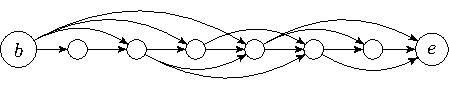
\includegraphics[scale=1.0]{img/unoptimized-graph.pdf}
  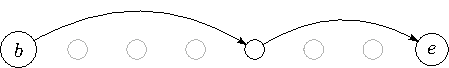
\includegraphics[scale=1.0]{img/optimized-graph.pdf}
  \caption{Optimal node subset using the graph approach}
\end{figure}


\section{EXPERIMENTS}
We can talk about the offline optimisation we did on some dataset.

\begin{figure}
  \caption{Comparison of un-optimized and optimized maps}
\end{figure}


\section{FUTURE WORK}

\begin{itemize}
  \item Experiment with Husky

  \item Multi objective optimization to have an automatic error elipse

  \item handling rotations (3D ellipsoid)

  \item Reoptimisation of the graph

\end{itemize}

\subsection{Multi-objective optimization for automatic parameter selection}

\subsection{Handling of rotations}

For the sake of simplicity we did not use rotations when inducing errors to the reading's
position estimate, before testing the reliability of the localization. To make the optimization
problem more difficult, while giving the user more ways garantee the reliability of the optimized
maps, we could replace $T$ the space of translations with $R \times T$ the space of rotations and
translations in function $f$. That way, the user could demand that the generated maps be tolerant to
a certain error in the orientation of the robot.

Using the whole space of rotations $R$ might be too general, as it is often useful to simplify the pose of a
ground robot begin a vector $[x, y, \theta]^t$, $\theta$ being the heading. That case could also be
handled by replacing the tolerance ellipse by an ellipsoid. The supplementary dimension would
represent the error in heading, or $\Delta \theta$.

\subsection{Reoptimization of the localizability graph}



\section{CONCLUSION}

\end{document}
